% !TeX spellcheck = fr_FR
%%%%%%%%%%%%%%%%%%%%%%%%%%%%%%%%%%%%%%%%%%%%%%%%%%%%%%%%%%%%
\chapter{Précisions sur Latex}
\label{chap:latex}
%%%%%%%%%%%%%%%%%%%%%%%%%%%%%%%%%%%%%%%%%%%%%%%%%%%%%%%%%%%%

L'annexe courante donne des exemples (voir fichier \texttt{annexes/annexe-SpecLatex.tex}) pour utiliser différents paquets inclus dans la classe. 

\section{Abbréviations et accronymes}
%%%%%%%%%%%%%%%%%%%%%%%%%%%%%%%%%%%%%%%%%%%%%%%%%%%%%%%%%%%%

....

\section{Figures}
%%%%%%%%%%%%%%%%%%%%%%%%%%%%%%%%%%%%%%%%%%%%%%%%%%%%%%%%%%%%


Une figure devrait être dans un environnement flottant et préférablement positionnée en haut ou en bas de page (option de positionnement \texttt{tb}) :

\begin{lstlisting}[nolol,numbers=none,frame=]
\begin{figure}[tb]
	\centering
	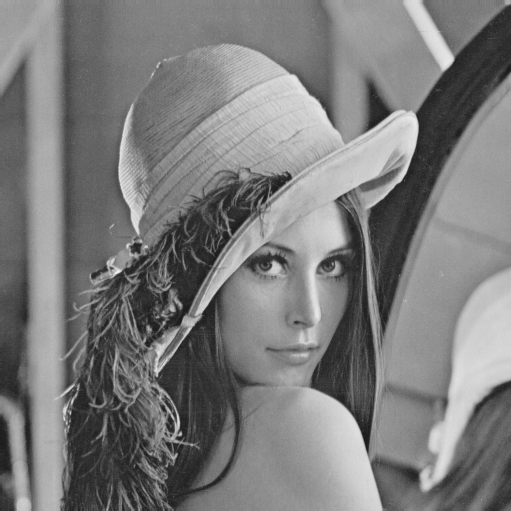
\includegraphics[width=0.45\linewidth]{lena.png}
	\caption[Titre pour la liste des figures]{On pourra mettre ce qu'on veut sous la figure, le titre dans la table des figures demeurera court.}
	\figlabel{figureSeule}
\end{figure}
\end{lstlisting}

\begin{figure}[tb]
	\centering
	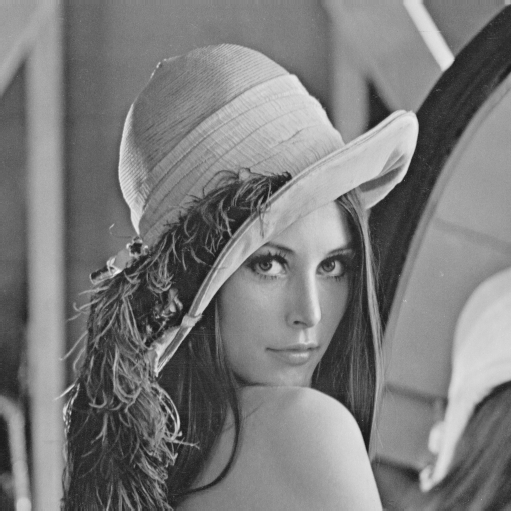
\includegraphics[width=0.45\linewidth]{lena} 
	\caption[Titre pour la liste des figures]{On pourra mettre ce qu'on veut sous la figure, le titre dans la table des figures demeurera court.}
	\label{fig:figureSeule}
\end{figure}

Le paquet \texttt{subfigure} vous permet d'avoir plusieurs images dans la même figure et des légendes différentes pour chacune. Vous pourrez référer à la figure entière ou à chaque sous-figure individuelle. Seul le titre principal de la figure se retrouvera dans la liste au début du document.

% \begin{figure}[t] 
% 	\centering
% 	\subfigure[Image du caméraman]{\label{subfig:camera}	
% 		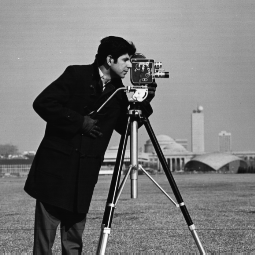
\includegraphics[width=0.25\linewidth]{camera.png}}
% 	\subfigure[Image de Lena]{\label{subfig:lena}
% 		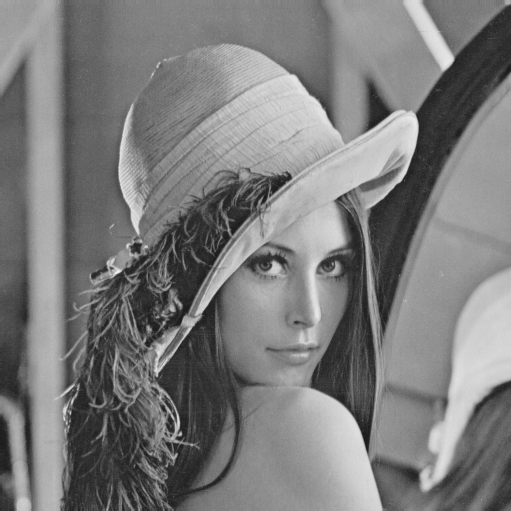
\includegraphics[width=0.25\linewidth]{lena.png}}
% 	\caption[Exemple d'inclusion de sous-figures]{Exemple d'inclusion de figures avec
% 		deux sous-figures pouvant avoir des légendes indépendantes. Elles peuvent être référencées de façon individuelles (voir \secref{refs}).} \label{fig:twoImages}
% \end{figure}

\clearpage

Des fois, latex accumule les éléments flottants avant de les placer dans le document et cela peut causer des problèmes. Il est bon de mettre la commande \verb|\clearpage| de temps en temps pour que les éléments flottants soient affichés dans les prochaines pages.

\section{Équations}
%%%%%%%%%%%%%%%%%%%%%%%%%%%%%%%%%%%%%%%%%%%%%%%%%%%%%%%%%%%%

Exemple d'une équation référencée dans le texte~:
\begin{equation}\label{eq:heatConserv}
	\nabla \cdot (\kappa \nabla u) = f.
\end{equation}

La suivante ne l'est pas alors on ne la numérote pas~:
\begin{equation*}
	\vec{v}(X,t)
	= \frac{dx}{dt} = \vec{v}(x,t).
\end{equation*}

\section{Tableaux}
%%%%%%%%%%%%%%%%%%%%%%%%%%%%%%%%%%%%%%%%%%%%%%%%%%%%%%%%%%%%

Le paquet \texttt{booktabs} vous permet de faire des tableaux plus agréables à l'oeil (voir \tabref{table1} et \url{https://www.ctan.org/pkg/booktabs} pour la documentation).

\begin{table}
	\centering
	\begin{tabular}{c c c}
		\toprule
		\textbf{Image}   & \textbf{Hello}   & \textbf{World}\\
		\hline
		\textbf{Ex1}  & $32$                  & 13.55 \\
		\textbf{Ex2}    & $5$                   & 48.20    \\
		\textbf{Ex3}    & $113$                 & 12.06    \\
		\bottomrule
	\end{tabular}
	\caption[Exemple d'un beau tableau]{Exemple d'un beau tableau avec un long
		titre.} \label{tab:table1}
\end{table}

\section{Légendes}
\label{sec:legendes}
%%%%%%%%%%%%%%%%%%%%%%%%%%%%%%%%%%%%%%%%%%%%%%%%%%%%%%%%%%%%


Utilisez l'option \texttt{Titre court} de \texttt{caption} pour éviter les noms trop longs dans les listes des pages préliminaires du document~:

\begin{verb}
	\caption[Titre court]{Titre long}
\end{verb}.

remarque faire la liste des préfixes à utiliser pour utiliser autoref et refstyle.

\section{Étiquettes}
\label{sec:etiq}
%%%%%%%%%%%%%%%%%%%%%%%%%%%%%%%%%%%%%%%%%%%%%%%%%%%%%%%%%%%%

Le paquet \texttt{refstyle} permet de faciliter la manipulation des étiquettes et surtout des références croisées (voir \secref{refs}). 

Afin de permettre une utilisation optimale des références croisées faciles, il est de requis de préfixer chaque étiquette du type d'élément à laquelle elle fait référence (\url{https://en.wikibooks.org/wiki/LaTeX/Labels_and_Cross-referencing#cite_note-:0-6}).

Voici les types qui sont définis et dont la version française est fournie pour utiliser \texttt{refstyle} :

\begin{itemize}
	\item[part:] partie
	\item[chap:] chapitre ou annexe
	\item[sec:]  section
	\item[subsec:] subsection
	\item[fig:] figure
	\item[subfig:] sous-figure
	\item[tab:] tableau
	\item[eq:] équation
	\item[lst:] recopie de code
	\item[itm:] item d'une liste
	\item[algo:] algorithme
	\item[fn:] note de bas de page
\end{itemize}

Voir aussi les différentes sections de cette annexe pour des exemples d'étiquettage vous permettant d'utiliser le paquet \texttt{refstyle} correctement.

\newpage

\section{Algorithmes}
%%%%%%%%%%%%%%%%%%%%%%%%%%%%%%%%%%%%%%%%%%%%%%%%%%%%%%%%%%%%

Voici un exemple d'algorithme entré dans l'environnement \texttt{algorithmic} dont les mots-clés seront en français si le document est en français. Vous pouvez adapter ou enlever la francisation dans le document \texttt{ajoutsFct.tex}.

\begin{algorithm}[H]
	\caption[Titre court]{Algorithme avec étiquette trop longue pour la liste du début}\label{algo:cap}
	\begin{algorithmic}
		\Require $n \geq 0$
		\Ensure $y = x^n$
		\State $y \gets 1$
		\State $X \gets x$
		\State $N \gets n$
		\While{$N \neq 0$}
		\If{$N$ is even}
		\State $X \gets X \times X$
		\State $N \gets \frac{N}{2}$  \Comment{commentaire}
		\ElsIf{$N$ is odd}
		\State $y \gets y \times X$
		\State $N \gets N - 1$
		\EndIf
		\EndWhile
	\end{algorithmic}
\end{algorithm}

\clearpage

\section{Codes sources}
%%%%%%%%%%%%%%%%%%%%%%%%%%%%%%%%%%%%%%%%%%%%%%%%%%%%%%%%%%%%

% https://en.wikibooks.org/wiki/LaTeX/Source_Code_Listings
%\lstset{language=C++}  % en dehors de l'environnement lstlisting
%\lstset{}

Il est possible de mettre des recopies de codes sources dans votre document. 

Voir \url{https://en.wikibooks.org/wiki/LaTeX/Source_Code_Listings} pour plus d'information sur le paquet \texttt{lstlisting} dont vous avez quelques exemples d'utilisation ici.

Préférez l'inclusion des codes assez courts (moins d'une page) dans des environnements flottants. Sinon, le code sera traité comme du texte concernant le placement, à privilégier pour du code plus long qu'une page. Cette dernière option devrait être utilisée avec parcimonie.

\begin{lstlisting}[
	language=Python, 
	caption={[Titre court du code] Ceci est un code en C++ écrit directement dans le fichier \texttt{.tex}},
	label=lst:tex,
	% autres options disponibles
]
import numpy as np

def incmatrix(genl1,genl2):
	m = len(genl1)
	n = len(genl2)
	M = None #to become the incidence matrix
	VT = np.zeros((n*m,1), int)  #dummy variable
	
	#compute the bitwise xor matrix
	M1 = bitxormatrix(genl1)
	M2 = np.triu(bitxormatrix(genl2),1) 
	
	for i in range(m-1):
		for j in range(i+1, m):
			[r,c] = np.where(M2 == M1[i,j])
			for k in range(len(r)):
				VT[(i)*n + r[k]] = 1;
				VT[(i)*n + c[k]] = 1;
				VT[(j)*n + r[k]] = 1;
				VT[(j)*n + c[k]] = 1;
	
				if M is None:
					M = np.copy(VT)
				else:
					M = np.concatenate((M, VT), 1)
				
				VT = np.zeros((n*m,1), int)
	
	return M
\end{lstlisting}

\begin{lstlisting}[
	float, 			% environnement flottant
	language=c++ ,
	caption=A floating example, 
	nolol,    % enlève l'entrée de la liste des codes sources.
]
Carte::Carte(unsigned int i_nDim) :
m_nDimension{i_nDim}
{
	// Creation du tableau des valeurs
	vector<unsigned int> vecColonne (i_nDim, 0);
	m_tab.assign(i_nDim, vecColonne);
	m_nNbCasesVides = m_nDimension * m_nDimension;
	unsigned int premierChiffre ;
	premierChiffre = genereChiffre(Direction(random::genereValeur(0, 3)));
	m_nMax = premierChiffre;
};
\end{lstlisting}

\lstinputlisting[
	float, 					% environnement flottant
	caption={Code en python inclus en partie à partir d'un fichier dans un float},
	label=lst:incl, 
	language=Python, 
	firstline=2, lastline=12, % première et dernière ligne à inclure
]{annexes/exempleCodePython.py}

\clearpage

\lstinputlisting[
	caption={Code en python inclus à partir d'un fichier mais pas dans un float},
	label=lst:nonfloat, 
	language=Python,
]{annexes/exempleCodePython.py}

\section{Références croisées}
\label{sec:refs}
%%%%%%%%%%%%%%%%%%%%%%%%%%%%%%%%%%%%%%%%%%%%%%%%%%%%%%%%%%%%

Vous pouvez toujours utiliser la façon régulière de faire vos références croisées, en utilisant simplement \verb@\ref{etiquette}@, \verb|\nameref{etiquette}| \\
ou \verb@\pageref{etiquette}@.

\begin{quote}
	Les chapitres \ref{chap:chapitre1} et \ref{chap:soumis}. Le nom du chapitre de conclusion est \nameref{chap:conclusion} et sa page est \pageref{chap:conclusion}. 
\end{quote}

Vous avez aussi deux façons alternatives: les références automatiques (\subsecref{autoref}) et l'utilisation de \texttt{refstyle} (\subsecref{refstyle}).

\subsection{Références automatiques}
\label{subsec:autoref}
%%%%%%%%%%%%%%%%%%%%%%%%%%%%%%%%%%%%%%%%%%%%%%%%%%%%%%%%%%%%

%\modeFrancais

Il est possible d'obtenir des liens plus lisibles (incluant le type d'objet dans le lien) avec \texttt{autoref}. La traduction du terme est automatique aussi.
Par exemple :

\begin{quote}
Le \autoref{chap:chapitre1} et le \autoref{chap:soumis}. La page du chapitre de conclusion est \autopageref{chap:conclusion}.

Pour les différents éléments, la commande choisit le meilleur terme : \autoref{chap:latex}, \autoref{eq:heatConserv}, \autoref{fig:figureSeule}, \autoref{lst:incl}, \autoref{sec:abbrev}, \autoref{subsec:autoref}, \autoref{tab:table1}, \autoref{algo:cap}.
\end{quote}

Ceci est à comparer à
\begin{quote}
	Le chapitre \ref{chap:chapitre1} et le chapitre \ref{chap:soumis}. La page du chapitre de conclusion est \pageref{chap:conclusion}.
	
	Pour les différents éléments, la commande ne choisit pas le meilleur terme, il faut l'ajouter explicitement : annexe \ref{chap:latex}, équa. \ref{eq:heatConserv}, Figure \ref{fig:figureSeule}, code \ref{lst:incl}, section \ref{sec:abbrev}, sous-section \ref{subsec:autoref}, tableau \ref{tab:table1}
\end{quote}

\subsubsection{Désavantages}

La commande \texttt{autoref} pose certains désavantages, elle n'offre pas un niveau de contrôle élevée : 

\begin{itemize}
	\item Il n'y a pas de contrôle sur la première lettre qui ne peut se mettre en majuscule.
	\item On ne peut pas mettre plusieurs étiquette dans la même commande.
\end{itemize}

Le paquet \texttt{refstyle} remédie à ces problèmes mais n'offre pas la possibilité d'inclure le nom de l'élément dans le lien sauf pour les chapitres et annexes.

\subsection{Utilisation de \texttt{refstyle}}
\label{subsec:refstyle}
%%%%%%%%%%%%%%%%%%%%%%%%%%%%%%%%%%%%%%%%%%%%%%%%%%%%%%%%%%%%

Pour bien utiliser \texttt{refstyle}, il faut étiqueter correctement les éléments en utilisant les préfixes par type (voir \secref{etiq}).
Par exemple la référence à l'équation étiquetée \texttt{eq:HeatConserv} indique que l'élément est une équation. Si on utilise \verb|\eqref{HeatConserv}| (notez le passage du préfixe de l'étiquette vers un préfixe équivalent de la commande de référence, sans les «:»), on inclue le type de l'élément dans la référence.

Pour les différents éléments, la commande choisit le terme à inclure dépendamment du préfixe de la commande.
\begin{quote}
	Le \chapref{chapitre1} et le \chapref{soumis}. 
	
	\chapref{latex}, \eqref{heatConserv}, \figref{figureSeule}, \lstref{incl}, \secref{abbrev}, \subsecref{autoref}, \tabref{table1}, \algoref{cap}
\end{quote}

Il est possible de mettre la première lettre en majuscule : \Eqref{heatConserv}.

Le pluriel ainsi que les mots de liens se font automatiquement en mettant plusieurs étiquettes du même type,  séparées par des virgules, dans la référence.

Dans la \figref{twoImages}, nous avons deux images, c'est-à-dire, les \subfigref{camera, lena}.

Le no. de page : \subfigpageref{camera}. 

Le nom de la section contenant un élément \nameref{algo:cap}.

Référence à la \secref{legendes}. Référence aux \subsecref{refstyle, three}.

Références aux \subsecref{autoref, refstyle, three} ou aux \lstrangeref{tex}{nonfloat} .

\subsection{Langue des références dans le texte}
\label{subsec:three}
%%%%%%%%%%%%%%%%%%%%%%%%%%%%%%%%%%%%%%%%%%%%%%%%%%%%%%%%%%%%

Il est possible de changer le mode de langue pour passer à l'anglais (utilisation de \verb|\modeAnglais|, \verb|\modeFrancais|, \verb|\modeDefaut|) autant avec \texttt{autoref} qu'avec \texttt{refstyle}.

On passe au mode anglais (\verb|\modeAnglais|).
\modeAnglais

\begin{quote}
	\texttt{autoref}:
	
	Le \autoref{chap:chapitre1} et l'\autoref{chap:latex}. La page du chapitre de conclusion est \autopageref{chap:conclusion}. Autres exemples : \autoref{eq:heatConserv}, \autoref{fig:figureSeule}, \autoref{lst:incl}, \autoref{sec:abbrev}, \autoref{subsec:autoref}, \autoref{tab:table1}.
	
	\texttt{refstyle}:
	
	Le \chapref{chapitre1} et le \chapref{latex}. Autres exemples : \eqref{heatConserv}, \figref{figureSeule}, \lstref{incl}, \secref{abbrev}, \subsecref{autoref}, \tabref{table1}, \algoref{cap}, \Eqref{heatConserv}, \subfigref{camera, lena}, \subfigpageref{camera}, \subsecref{autoref, refstyle, three}, \lstrangeref{tex}{nonfloat}.
\end{quote}

On revient au mode français (\verb|\modeFrancais|) .
\modeFrancais

\begin{quote}
		\texttt{autoref}:
	
	Le \autoref{chap:chapitre1} et l'\autoref{chap:latex}. La page du chapitre de conclusion est \autopageref{chap:conclusion}. Autres exemples : \autoref{eq:heatConserv}, \autoref{fig:figureSeule}, \autoref{lst:incl}, \autoref{sec:abbrev}, \autoref{subsec:autoref}, \autoref{tab:table1}.
	
	\texttt{refstyle}:
	
	Le \chapref{chapitre1} et l'\chapref{latex}. Autres exemples : \eqref{heatConserv}, \figref{figureSeule}, \lstref{incl}, \secref{abbrev}, \subsecref{autoref}, \tabref{table1}, \algoref{cap}, \Eqref{heatConserv}, \subfigref{camera, lena}, \subfigpageref{camera}, \subsecref{autoref, refstyle, three}, \lstrangeref{tex}{nonfloat}.
\end{quote}

\modeDefaut

\section{Abréviations}
\label{sec:abbrev}
%%%%%%%%%%%%%%%%%%%%%%%%%%%%%%%%%%%%%%%%%%%%%%%%%%%%%%%%%%%%

Si vous avez des définitions d'abréviations utilisant\\
\begin{verb}
	\newabbreviation{etiquette}{ABR}{Expression à remplacer},
\end{verb}\\
il devient facile d'insérer rapidement celles-ci dans le texte avec seulement l'étiquette en utilisant \verb|\gls{etiquette}|. À la première utilisation, elle sera automatiquement étendue avec l'abbréviation entre parenthèses.
\begin{quote}
	\gls{etiquette}, vs \gls{etiquette} vs \glsentryfull{etiquette}.
\end{quote}

Voir \url{https://en.wikibooks.org/wiki/LaTeX/Glossary} pour plus de détails.
